\section{Introduction}
\label{sec:intro}
Generic image segmentation has been part of computer vision and image processing communities since the
advent of these fields many decades ago.
The definition of the problem, although vague, is easy to give and understand: ``to divide the pixels of an
image into different pieces, where each piece represents a distinguished \textit{thing}
in the image.''
Martin \etal~\cite{Martin2001} provided these instructions to annotators to create
the Berkeley Segmentation Database (BSDS), which proved that the problem of image segmentation was,
indeed, well defined, as humans provided consistent partitions of the images \textit{up to refinement}.
In other words, image segmentation is inherently a multi-scale problem.

We refer to \textit{flat} image segmentation techniques as those whose output is a single partition of the
image pixels into sets~\cite{shi2000normalized,Comaniciu2002,felzenszwalb2004efficient}.
In these cases, in order to capture the aforementioned multi-scale nature of objects,
one needs to sweep different parameterizations to obtain multiple partitions that contain the
different scales when working with flat segmentation techniques.

On the other hand, hierarchical segmentation produces a single multi-scale structure that aims
at capturing the objects at all scales~\cite{arbelaez2011contour,kim2013learning,Salembier2000,Ren2013,arbelaez2014multiscale}. 
These types of structures have been successfully used in image filtering~\cite{Salembier2000},
semantic segmentation~\cite{Lempitsky2011}, object proposals generation~\cite{arbelaez2014multiscale},
or video segmentation~\cite{xu2013flattening,Varas2015}.

\begin{figure}
\begin{center}
\begin{minipage}{0.24\linewidth}
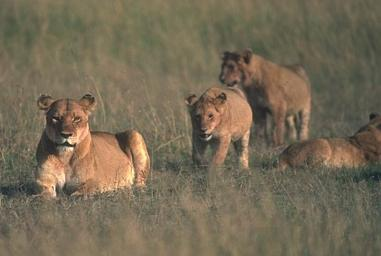
\includegraphics[width=\linewidth]{fig/aligned_lions/cropped_image.jpg}
\end{minipage}
\begin{minipage}{0.24\linewidth}
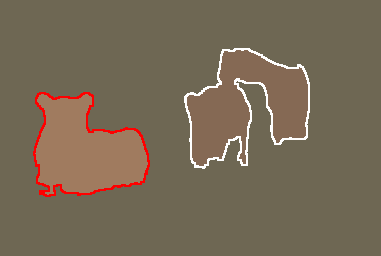
\includegraphics[width=\linewidth]{fig/aligned_lions/mcg_underseg.png}\\[1mm]
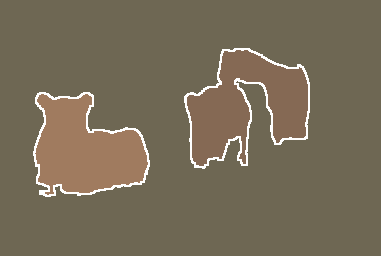
\includegraphics[width=\linewidth]{fig/aligned_lions/mcg_our_underseg.png}
\end{minipage}
\begin{minipage}{0.24\linewidth}
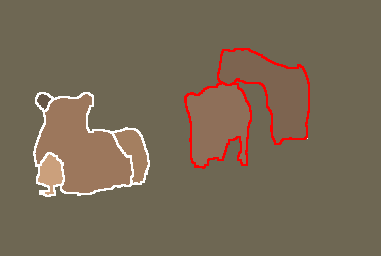
\includegraphics[width=\linewidth]{fig/aligned_lions/mcg_mid.png}\\[1mm]
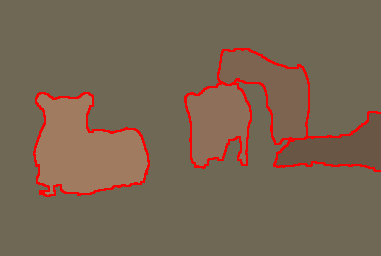
\includegraphics[width=\linewidth]{fig/aligned_lions/mcg_our_good.png}
\end{minipage}
\begin{minipage}{0.24\linewidth}
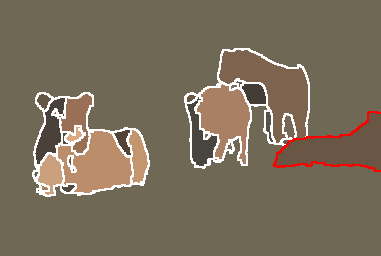
\includegraphics[width=\linewidth]{fig/aligned_lions/mcg_overseg.png}\\[1mm]
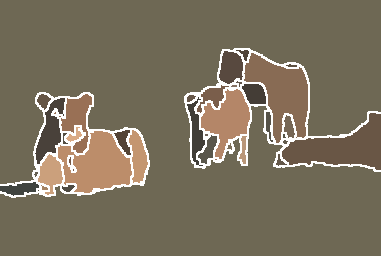
\includegraphics[width=\linewidth]{fig/aligned_lions/mcg_our_overseg.png}
\end{minipage}
\end{center}
\vspace{-2mm}
\caption{\textbf{Example of improved hierarchy alignment}: The original hierarchy (top row) needs three
different flat partitions to represent the four objects (highlighted in red).
Our aligned hierarchy (bottom row) correctly puts all objects in the same level.}
\vspace{-2mm}
\label{fig:thresh_seg}
\end{figure}

The representation power of these hierarchies comes at a cost, however, which is the
difficulty to handle them from a practical (coding) point of view.
While a flat partition can be represented by a matrix of labels of each pixel,
hierarchical structures need a much more complex representation. 
In this context, the Ultrametric Contour Map (UCM)~\cite{arbelaez2011contour} representation is the one that 
gained more traction and it is widely used in the literature.
In it, \textit{flattening} the hierarchy can be achieved by simply \textit{thresholding} the UCM.

The process of \textit{flattening} or \textit{pruning} a hierarchy is therefore of paramount importance for
segmentation, because it is the main proxy used towards the final application.
This work presents a novel technique to improve the flattening of any given hierarchy, that is, 
to get better flat partitions from the same hierarchical segmentation.

\begin{figure*}
\begin{center}
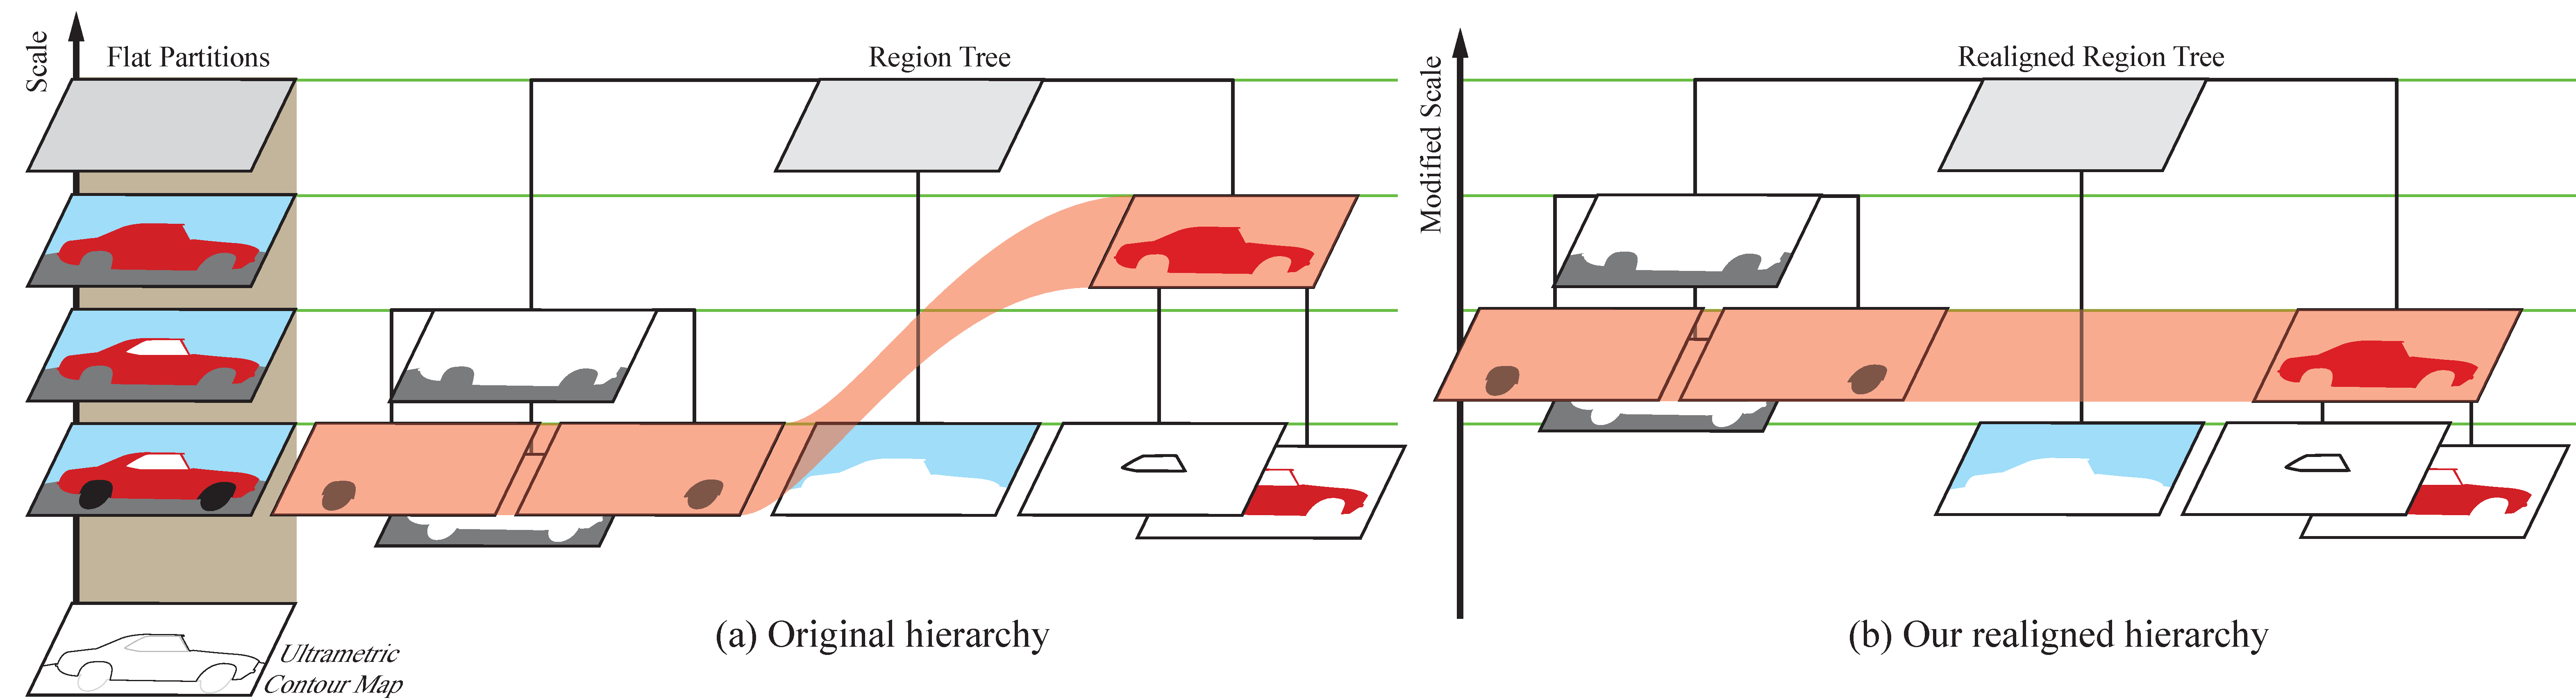
\includegraphics[width=\textwidth]{fig/hierarchy.pdf}
\end{center}
\vspace{-2mm}
\caption{\textbf{Our proposed hierarchy realignment}: Given a hierarchy (a) in which the objects at the same scale are not well aligned (represented in the same scale level), we produce a realigned hierarchy (b) that
has the similar-scale regions in the same level.}
\label{fig:hier_align}
\end{figure*}

Figure~\ref{fig:thresh_seg} motivates this work.
In the first row we can see different flat partitions extracted from the same hierarchy.
To get the regions representing the four lions we need to search in three different flat partitions, 
extracted at three different levels of the hierarchy.
The second row shows our results, where the same hierarchy is \textit{aligned} to have all objects represented in the same flat partition.

In other words, the threshold level of the hierarchy better relates with the scale of the objects, not only
in the same image, but also across images.
To further grasp the intuition of our work, Figure~\ref{fig:hier_align} shows a UCM and its interpretation as
a region tree (a).
In it, the needed regions to form the car are spread into different scale levels (thresholds of the UCM), as
marked by the red band.
Our proposed realigned hierarchy (b) aims at containing them all in the same scale.

Since the hierarchies are constructed based on low-level features (edges or color), the scale of the objects
is not imposed to be coherent.
We propose to learn the concept of object scale from mid-level features within the hierarchy.
Our objective is to take advantage of these mid-level features as much as possible without getting to
high-level features that would allow us to go beyond scale.
This way, the global approach would be to construct the hierarchies using low-level features,
and then exploit mid-level features to realign them, thus taking the maximum advantage of the most simple 
features possible.

Our alignment also aims at providing a global alignment among different images, that is, providing levels 
of scale that keep meaning even when changing images, allowing higher-level methods to generalize in a more straightforward manner.
Specifically, we train a regressor to predict whether each region of the hierarchy is oversegmented, undersegmented, or correctly segmented; and we rescale the hierarchy according to the prediction 
of this classifier.
Back to the example in Figure~\ref{fig:thresh_seg}, the majority of regions in the first column (bottom) 
are undersegmented, in the middle column they are correctly segmented, and oversegmented in the last column.

We perform comprehensive experiments on BSDS500 using four different hierarchical segmenters.
We obtain consistent improvements on all hierarchies which proves the usefulness of our approach and its 
generalization power.
The remainder of the paper is organized as follows.
First, Section~\ref{sec:related} gives a brief overview of the related work.
Then Section~\ref{sec:scaling} presents our algorithm for re-scaling and aligning hierarchies.
We demonstrate the effectiveness of our method in the experiments in Section~\ref{sec:experiments} and draw 
the conclusions in Section~\ref{sec:conclusions}.
 
%\yh{following is the old introduction}

%Hierarchical segmentation decomposes a given image into a hierarchy of regions, with the constriant that regions in the lower level are the subparts of higher level. Hierarchical segmentation is commonly represented as an ultrametric contour map (UCM), where different levels of segmentation can be produced by applying certain threshold to UCM. Flat segmentation can be extracted by thresholding the UCM at different scales.
%
%For many vision applications, an input of flat segmentation is required\todo{add some refs}. Thus how to choose proper threshold becomes an important issue. Threshold chosen improperly may result in unsatisfactory segmentation. As can be seen from Fig~\ref{fig:thresh_seg}, too fine a scale will break a region into many small pieces, too coarse a scale will mix different regions together. A common practice is to fix an optimal-dataset-scale(ODS) beforehand based on a group of training images. However, in practice it is unlikely that a single setting of parameters will produce best segmentation result for any general images. In order to achieve optimal result, it takes significant amount of human efforts to tune optimal-image-scale(OIS) for each image. Besides, in some case, no single segmentation is capable of capturing all the regions. For example, there are four lions in Fig~\ref{fig:fail_seg}. Each single segmentation can capture one or two lion. But all the segmentations failed no matter how to choose the scale. 
%
%Though its siginificant importance, the problem of how to flatten a hierarchy into a flat segmentation has long been ignored. In this work, instead of choosing one optimal scale, we aim to take leverage of the rich multiscale information stored in the segmentation hierarchy.  The key idea of our work is to save all the good segments in different scale, and combine them into a single segmentation. Specifically, we learn to identify a group of potential scale that may includes useful regions for each specific image. Then we make use of mid-level and high level features to predict the quality of regions. In order to flatten segmentation hierarchies, we develop a simple and efficient algorithm to merge different scales greedily based on the score predicted before.
%
%We conduct extensive experiments on the BSDS500 dataset, and NYC dataset~\todo{add later}.   

% The underlying assumption is that there is a common parameter for all the images. However, the assumption barely holds in practice due to large diversity in natural images. Another 




